%%%%%%%%%%%%%%%%%%%%%%%%%%%%%%%%%%%%%%%%%%%%%%%%%%%%%%%%%%%%%%%%%%%%%%%%
%                                                                      %
%     File: Thesis_Background.tex                                      %
%     Tex Master: Thesis.tex                                           %
%                                                                      %
%     Author: Andre C. Marta                                           %
%     Last modified :  2 Jul 2015                                      %
%                                                                      %
%%%%%%%%%%%%%%%%%%%%%%%%%%%%%%%%%%%%%%%%%%%%%%%%%%%%%%%%%%%%%%%%%%%%%%%%

\chapter{Background}
\label{chapter:stateoftheart}


To reflect the recent GPUs use cases and the efforts being made in the pursuit of improving the performance and minimizing the energy consumption of them, this chapter provides an overview of modern GPUs architecture, with a brief specialization on the AMD GNC architecture. It also presents what kind of power savings techniques are currently being employed in existent hardware, and a review of the literature related to the effects that changing the frequency and voltage. The relevance of this work emerges from the reduce number of studies on the effects of voltage scaling on GPUs, being that, one of the objective of this dissertation. This is due to lack of support for control of this parameter on NVIDIA GPUs (until recently, the dominent player on the market \cite{noauthor_jon_nodate} \cite{mujtaba_amd_2019}) that is now allowed by the novel AMD software stack used on this work. Furthermore, an overview of power and performance models is provided, highlighting the different techniques used to predict these two metrics. 


%%%%%%%%%%%%%%%%%%%%%%%%%%%%%%%%%%%%%%%%%%%%%%%%%%%%%%%%%%%%%%%%%%%%%%%%
\section{General Purpose Computing on GPUs}
\label{section:gpuarch}

A GPU is a highly parallel programmable processor, that is built to perform the same instruction on a set of data, belonging to the category of processors of \textit{Single Instruction Multiple Threads} - SIMT. When referring to GPUs, it is still common to be talking about their graphics capabilities, however, more and more programs are taking advantage of their highly parallel architecture to accelerate applications. The use of GPUs in general programming commonly referred to as GPGPU - General Purpose Graphical Processing Unit was first led by the development of CUDA \cite{noauthor_cuda_2017} by NVIDIA and OpenCL \cite{noauthor_opencl_2013} by Khronos Group. CUDA and OpenCL are both parallel computing platforms and application programming interface (API) that allows developers to create GPU-accelerated applications, where the computations can be divided between the CPU and GPU. The first versions of these frameworks treated the GPU as a slave device, providing a set of directives that allow the CPU (master device) to transfer data, synchronize and control the GPU.  Though, to take full advantage of the GPU architecture and create a true heterogeneous system, the CPU and GPU collaborate more efficiently. This lead to, in 2012, the proposal by the HSA Foundation for the creation of a Heterogeneous System Architecture (HSA) \cite{hwu_heterogeneous_2015} framework that acts as an intermediary low-level API to provide improved coordination and communication for heterogeneous computing systems.  More recently, AMD introduced the Radeon Open Computing platform (ROC) \cite{noauthor_radeonopencompute/rocm_2019}. ROC, like CUDA and OpenCL, provides a set of tools that allow developers to create heterogeneous applications. The added benefits of ROC are that it is built on top of the HSA runtime API and it exposes the framework in a wider set of programming frameworks like OpenCL, HC++, and HIP.

The development of improved frameworks and programming methodologies are making GPUs the prime tool to accelerate deep learning applications. GPUs can outperform CPUs in both throughput and energy efficiency. In this section, it will be provided a general overview of the GPU architecture, followed by a presentation of the tools that are going to be used on the dissertation.


\subsection{General Overview of GPU Architecture}
The architecture of the GPU can be roughly divided into computation and memory components. The computation part is composed of the vertex shader, the rendering engine, and the RISC processors. The vertex shader and rendering engine are inserted on the graphics pipeline and are not generally used on GPGPU applications. The RISC processors are responsible for the GPU programmable calculations, and depending on the manufacturer, can be called streaming multiprocessors (SM) in NVIDIA GPUs \cite{nvidia_cuda_nodate} or computing units (CU) in AMD GPUs \cite{amd_amd_nodate}.  To enable concurrent execution of multiple threads in a single CU, each is made up of hundreds of execution units, and, in order for the threads to have low-overhead context switch, modern GPUs provide a large register file on each CU, where the context of all active threads can be stored. For reference, in the AMD GNC architecture, each CU has 49,152 (32-bit) registers \cite{jing_energy-efficient_2013}.

In terms of memory, both the AMD and the NVIDIA GPU present a 3 level hierarchy system: a global memory, accessible by all processors units (generally referred as video memory); a shared memory associated with each SM or CU, accessible by the threads running on that SM or CU; and a set of read-only caches for constants and textures, specific of each thread.

A GPU from AMD will be used to conduct the experimental part of this dissertation. For that reason, a more in-depth analysis of the architecture and framework from this manufacturer will be provided and, the terminology used by AMD will be adopted. However, the presented work is independent of the hardware and terminology itself.

\subsection{AMD Graphics Core Next}

The AMD Graphics Core Next (GCN) \cite{amd_radeons_nodate}  architecture includes both the GPU microarchitecture as well as the instruction set of the processor unit. The architecture was first released in 2012, and it is already in its fifth iteration with the codename Vega. The Vega microarchitecture is based on a multiprocessor chip with an array of 64 RISC SIMT processors called Compute Engine (CE). Respectively, each CE is constituted by 64 Next Compute Units (NCU), performing a total of 4096 Compute Units. The interface between the GPU and the host is done throw the Peripheral Compute Interconnect Express (PCIe). Figure \ref{fig:Vega10arch} represents the logical organization of a Vega GPU.  

\begin{figure}[!htb]
  \begin{subfigmatrix}{2}
    \subfigure[Chip block diagram, example with 4 CEs]{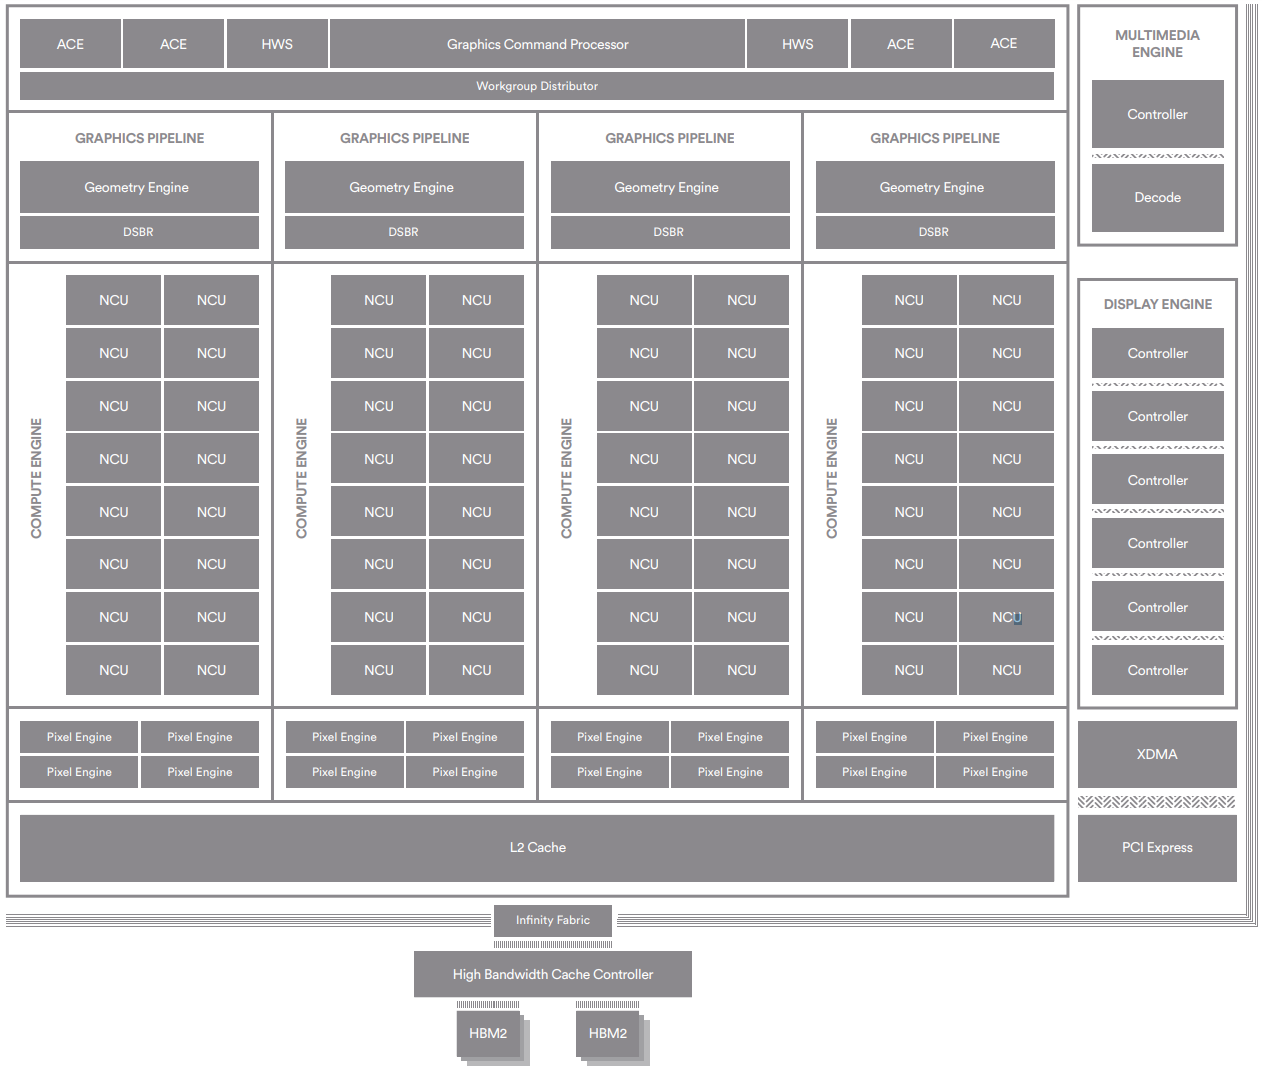
\includegraphics[width=0.7\linewidth]{Figures/StateArt/Vega10_microarchitecture.png}}
    \subfigure[NCU]{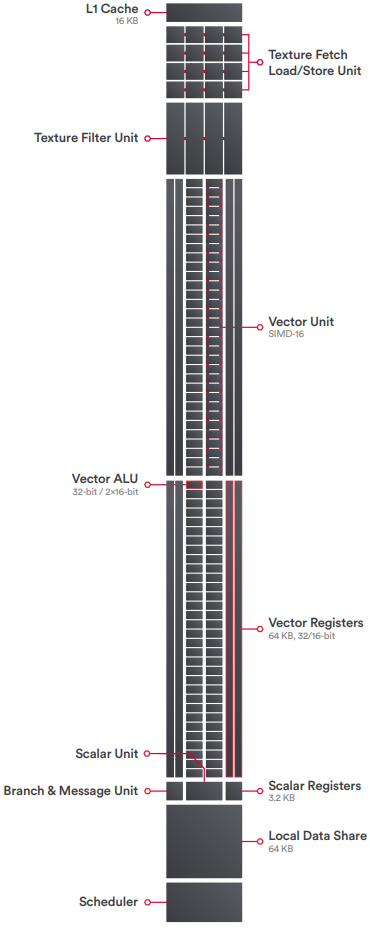
\includegraphics[width=0.24\linewidth]{Figures/StateArt/NCU.png}}
  \end{subfigmatrix}
  \caption{AMD's Graphics Core NExt logical Organization.}
  \label{fig:Vega10arch}
\end{figure}

In the fifth iteration of the GNC microarchitecture, AMD introduced a new memory hierarchy and support for High-Band Memory 2 (HBM2). In a conventional memory arrangement, the registers of each processing element pull data from a set of L1 caches, that, in turn, access the global L2 cache. Finally, the L2 cache system provides access to the GPU's video memory. This arrangement implies that the video memory has the entire working set of data and resources in order to provide high-bandwidth and low-latency access to data. However, in complex graphical scenes or while working GPGPU applications with large datasets, the total video memory may not be big enough to store all the data. In the Vega microarchitecture, by utilizing a  High-Bandwidth Cache Controller (HBCC), AMD made it possible to utilize the local video memory like a last-level cache. In this arrangement, when a missing piece of data, not currently stored in the local memory, is needed by the CUs, the GPU can pull just the necessary page memory from the host. In this setup, instead of the GPU stalling, while the entire missing resource is copied from the host throw the PCIe bus, it just needs to wait for the smaller page memory to be transferred, resulting in significantly decreased memory access times. The GPGPU applications take great advantage of this memory hierarchy since it enables the use of bigger datasets than the ones that could fit in the device video memory.

In the development of the work of this dissertation, a Radeon Vega Frontier Edition GPU is used. Table \ref{tab:gpusepcs} summarizes the most important specifications of the architecture of this device.

\begin{table}[!htb]
    \renewcommand{\arraystretch}{1.2} % more space between rows
    \centering
        \begin{tabular}{lc}
            \multicolumn{1}{c}{\textbf{}} & \multicolumn{1}{l}{\textbf{Radeon™ Vega Frontier Edition}} \\ \hline
            Base Architecture             & Vega GNC                                                   \\
            \#Compute Units               & 64                                                         \\
            \#Stream Processors           & 4096                                                       \\
            GPU Memory Size               & 16 GB                                                      \\
            Thermal Design Power          & 300 W                                                      \\ \hline
        \end{tabular}
    \caption{Characteristics of the used GPU device}
    \label{tab:gpusepcs}
\end{table}

\subsection{Radeon Open Compute platform}

The Radeon Open Compute (ROC) \cite{noauthor_radeonopencompute/rocm_2019} platform provides support for a set of frameworks and tools to allow developers to program and control the AMD GPUs. Figure \ref{fig:rocmplatform} shows the high-level organization of the platform. The platform includes a set of tools that allows developers to access ROC Kernel Driver data. In the following subsections, two of those tools, the ROCM-SMI \cite{noauthor_radeonopencompute/roc-smi_2019} and ROC-Profiler \cite{noauthor_rocm-developer-tools/rocprofiler_2019}, used on the development of this work, are described.

\begin{figure}[!htb]
  \centering
  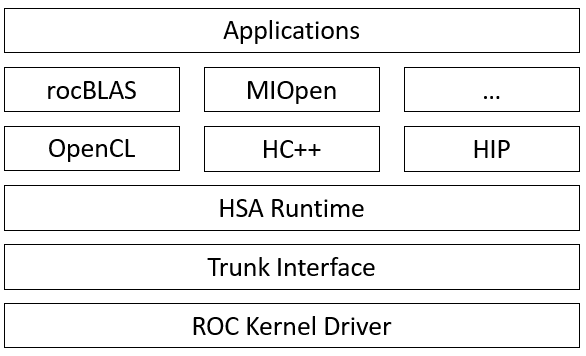
\includegraphics[width=0.5\textwidth]{Figures/StateArt/rocStack.png}
  \caption{Organization of the ROC platform.}
  \label{fig:rocmplatform}
\end{figure}

\subsubsection{ROCM-SMI}
The ROCm System Management Interface (ROC-SMI) \cite{noauthor_radeonopencompute/roc-smi_2019} is a user-friendly command-line application for manipulating the Radeon Open Compute Kernel (ROCK). By using it, it becomes possible to know and control the state of the GPU devices presented on the system. The application uses sysfs files to query and manipulate the device kernel using the libsensors library \cite{noauthor_libsensors3:_nodate}.

From the set of query and control directives enabled by ROC-SMI, the following are of particular interest for the topic of this dissertation:

\begin{itemize}
\item \textbf{GPU utilization:} Retrieves the current utilization rates for the device's major subsystems, one value for the processing core and other for the main device memory. The rate is computed over a specific time interval set on the libsensors library. The processing core utilization reflects the percentage of time that the GPU core was being utilized to perform computations. In contrast, the main device memory utilization reflects the percentage of time on which the memory was being read or written.

\item \textbf{GPU power}: Retrieves the average power used by the device. Similarly to the utilization rate, the average power computed over a defined time interval, during which a set number of power samples are taken.

\item \textbf{Clock rate and voltage level:} Retrieves both the currently applied clock frequency and voltage level to the GPU core and the main device memory. It also displays two tables, the first, showing the eight pairs of clock frequency/voltage level of the GPU core and the second, showing four pairs of the same parameters related to the device memory. These two tables, correspondent to the 8 and 4 performance levels that the device kernel can apply to the GPU core and memory correspondingly.
\end{itemize}

The ROC-SMI interface also allows querying the device temperature, the current fan speed, and the selected performance level.

ROC-SMI also provides a mechanism to control and change device parameters such as:
\begin{itemize}
\item \textbf{Set clock rate and voltage level:} Set the clock frequency and the voltage level of any of the performance levels of both the GPU core and memory. 
\item \textbf{Set performance level:} Allows the user to select the desired performance level of the GPU core and device memory, disabling the driver automatic performance level management system.
\item \textbf{Reset clock rate and voltage level:} Resets the clock rates and voltage level to the default values.
\end{itemize}

Additionally, the interface allows the user to manually set the fan speed, necessary to guarantee the same temperature level for all executed tests

The versatility and total and independent control of the clock rate and voltage level of the device allowed by ROCM-SMI and the libsensors library was the defining factor for choosing an AMD GPU over the more popular options of NVIDIA. In the development of the work presented in this dissertation, an exploration of the voltage level is undertaken, and only the AMD platform allows for independent control over this variable.

\subsubsection{ROC-Profiler}

The Radeon Open Compute Profiler \cite{noauthor_rocm-developer-tools/rocprofiler_2019} is a profiling and tracing library for applications developed using any of the programming frameworks available on the ROC platform (OpenCL, HC++, HIP) \cite{sun_evaluating_2018}. The library gives access to the performance counters of AMD GPUs, allowing developers to configure the start, stop, read and reset of the physical registers on the microarchitecture that count the number of events (number of instructions per type, cache hits/miss) that the device is performing.

The instrumentation of applications with the API calls to ROC-Profiler allows for close monitoring of the type of operations being performed. The use of this tool can give valuable insights about the relation of the running code and the utilized frequency and voltage, to the performance, power consumption and the results being produced.


%%%%%%%%%%%%%%%%%%%%%%%%%%%%%%%%%%%%%%%%%%%%%%%%%%%%%%%%%%%%%%%%%%%%%%%%


\section{Dynamic Voltage and Frequency Scaling}
\label{section:dcvf}

The widespread use of GPUs in both supercomputers and on personal machines comes at the cost of a significant increase in the power consumption of the complete system. Whereas a typical modern CPU consumes about 50 to 100W, it is common to see GPUs rounding that value to 200 to 300W of power. With these figures, it is indispensable the use of energy efficiency techniques to try to reduce power consumption.

On any CMOS circuit, the total power consumed is decomposed into the dynamic and static parts. The dynamic power relates to the act of the transistors flipping their stages, and correspond to the power of charging and discharging the internal net capacitances. This value is proportional to the frequency that this change occurs. Equation \ref{eq:dynpower} represents the general form for dynamic power, where \textit{a} represents the utilization factor, \textit{C} the total capacitance of the circuit, \textit{V} the transistors supplied voltage and \textit{f} the operating frequency \cite{gonzalez_supply_1997}.

\begin{equation}
    P_{dynamic} = aCV^2f
    \label{eq:dynpower}
\end{equation}


On their turn, the static part of the power consumption is generated by $P_{leakage}$, $P_{short-circuit}$ and $P_{DC}$ \cite{mei_survey_2016}. The leakage power is independent of the transistors flip, and it represents the flow of electrons between the transistors' source, drain, and gate, known as current leakage. The short-circuit power comes from the instantaneous short-circuit connection between the supply voltage and the ground when the transistor flips. Finally, the Direct Current (DC) power corresponds to the power needed for powering the circuit. Equation \ref{eq:cmospower} represents the total power consumption sources.

\begin{equation}
    P_{total} = P_{dynamic} + P_{leakage} + P_{short-circuit} + P_{DC}
    \label{eq:cmospower}
\end{equation}

The dynamic power dominates the total power consumption of a circuit, however, with the reduction of the manufacturing size of the transistor seen nowadays, the static power is also contributing heavily \cite{s._hong_modeling_2012} \cite{hong_integrated_2010}. As a common reference, due to the higher weight of the dynamic power on the total power consumption, the power used by a circuit changes linearly with the clock frequency and quadratically with the supplied voltage.

By intelligently controlling the clock frequency, the necessary voltage for stable operation of the circuit can also be reduced, leading to power savings. However, the reduction of the operating frequency harms the pic performance of the circuit, so a careful scaling of voltage/frequency needs to be done in run-time. The "on the fly" control of these parameters is called Dynamic Voltage and Frequency Scaling (DVFS). This power management technique allows for an energy efficiency improvement by matching the GPU utilization to the voltage and frequency apply to it.

In general, modern GPU boards have independent control over two pairs of frequency and voltage. Each pair or domain acts on a distinct part of the GPU, intending to maximize the performance or reduce the power consumption. The first domain concerns the GPU core, acting on all CUs, the cache, and the interconnection fabric. The second affects the DRAM chips that compose the video memory. 

The clock frequency is an independent control variable, and its change is reflected directly on the performed achieved by the GPU. An increase in the clock frequency of the core results in an improvement of the CU execution speed, while the same change in the memory frequency will increase the DRAM I/O throughput \cite{mei_survey_2016}. The voltage level of each domain is dependent on the clock frequency and is computed based on tests performed by the manufacturer that ensure the correct operation of the circuit, independently of the workload.

Both AMD and NVIDIA have on their products the concept of performance levels, that is, a set of pairs of frequency and voltage that can be applied to the many components of the GPU. These vary from low power and performance levels to high performance and high power ones. The idea of having multiple performance levels is to be able to always be at the best point of operation.  In the case of AMD, the GPU core has eight possible pairs, while the memory has only four. Table \ref{tab:gpulevels} shows the reference values for frequency and voltage for each of the core and memory performance levels. Through the use of software like ROC-SMI \cite{noauthor_radeonopencompute/roc-smi_2019} the user can input the desired combination of values for each level, allowing for an almost continuously selection of values for the frequency and voltage within the specifications range. For example, on the Vega 10 Frontier Edition, used on the experimental work of this thesis, the GPU core frequency can be set between 852 and 1980 MHz and the GPU memory frequency between 167 and 1500 MHz. In turn, the voltage can be set between the 800 and 1250 mV. As stated before, the primary benefit of AMD over NVIDIA's solution is that this manufacturer allows for the override of the automatic computation of the GPU voltage. This difference is of significant importance since it allows finer control of the DVFS values and a more interesting possibility of exploration of voltage scaling.


\begin{table}[!htb]
\renewcommand{\arraystretch}{1.2} % more space between rows
\centering
\begin{tabular}{ccclccc}
\multicolumn{3}{c}{\textbf{Core}}                                         & \multicolumn{1}{c}{\textbf{}} & \multicolumn{3}{c}{\textbf{Memory}}                                             \\
\textbf{Level} & \textbf{Frequency {[}MHz{]}} & \textbf{Voltage {[}mV{]}} &                               & \textbf{Level}       & \textbf{Frequency {[}MHz{]}} & \textbf{Voltage {[}mV{]}} \\ \cline{1-3} \cline{5-7} 
0              & 852                          & 800                       &                               & 0                    & 167                          & 800                       \\
1              & 991                          & 900                       &                               & 1                    & 500                          & 900                       \\
2              & 1138                         & 950                       &                               & 2                    & 800                          & 950                       \\
3              & 1269                         & 1000                      &                               & 3                    & 945                          & 1000                      \\ \cline{5-7} 
4              & 1348                         & 1050                      &                               & \multicolumn{1}{l}{} & \multicolumn{1}{l}{}         & \multicolumn{1}{l}{}      \\
5              & 1440                         & 1100                      &                               & \multicolumn{1}{l}{} & \multicolumn{1}{l}{}         & \multicolumn{1}{l}{}      \\
6              & 1528                         & 1150                      &                               & \multicolumn{1}{l}{} & \multicolumn{1}{l}{}         & \multicolumn{1}{l}{}      \\
7              & 1600                         & 1200                      &                               & \multicolumn{1}{l}{} & \multicolumn{1}{l}{}         & \multicolumn{1}{l}{}      \\ \cline{1-3}
\end{tabular}
\caption{GPU Core and Memory Levels of Frequency and Voltage - AMD Vega 10 Frontier Edition}
\label{tab:gpulevels}
\end{table}



\subsection{Control Mechanism}

The correct choice of the most appropriate performance level for each of the GPU clock domains is one of the topics of more research from both manufactures and researchers. The correct design of the DVFS controller has a significant impact on the performance and energy efficiency of the GPU.

The first implementations of GPU DVFS controllers took direct inspiration from the CPU DVFS and can be largely classified into interval-based, inter-task, and intra-task DVFS algorithms \cite{boyer_improving_2013}. 

\subsubsection{Interval-based}

Interval-based algorithms rely on the periodical measurement of the utilization of the device, setting the next frequency and voltage based on the average measurement of utilization. The utilization $U_{i}$ reflects the percentage of working time, $w_{i}$, spent by the GPU over the last time frame  $TF_{i}$ and can be formulated following equation \ref{eq:utilization}.

\begin{equation}
    U_i=\frac{w_i}{TF_i}
    \label{eq:utilization}
\end{equation}

By applying arithmetic, geometric, weighted average, or a more complex algorithm, over the last $n$ $U_{i}$ measurements,  the next utilization, $U_{i+1}$ is predicted. If the predicted value surpasses pre-determined upper or lower thresholds, the frequency is adjusted up or down accordingly \cite{seongki_gpgpu-perf:_nodate}. 
A \textit{governer} is a set of parameters such as frequency and voltage tables, thresholds and utilization prediction algorithm that controls how the interval-based DVFS works, by choosing a different \textit{governer}, the DVFS system can react differently to the same workload. Figure \ref{fig:DVFSprocedure} schematizes the periodic procedure executed by the DVFS system \cite{seongki_gpgpu-perf:_nodate}. 

\begin{figure}[!htb]
  \centering
  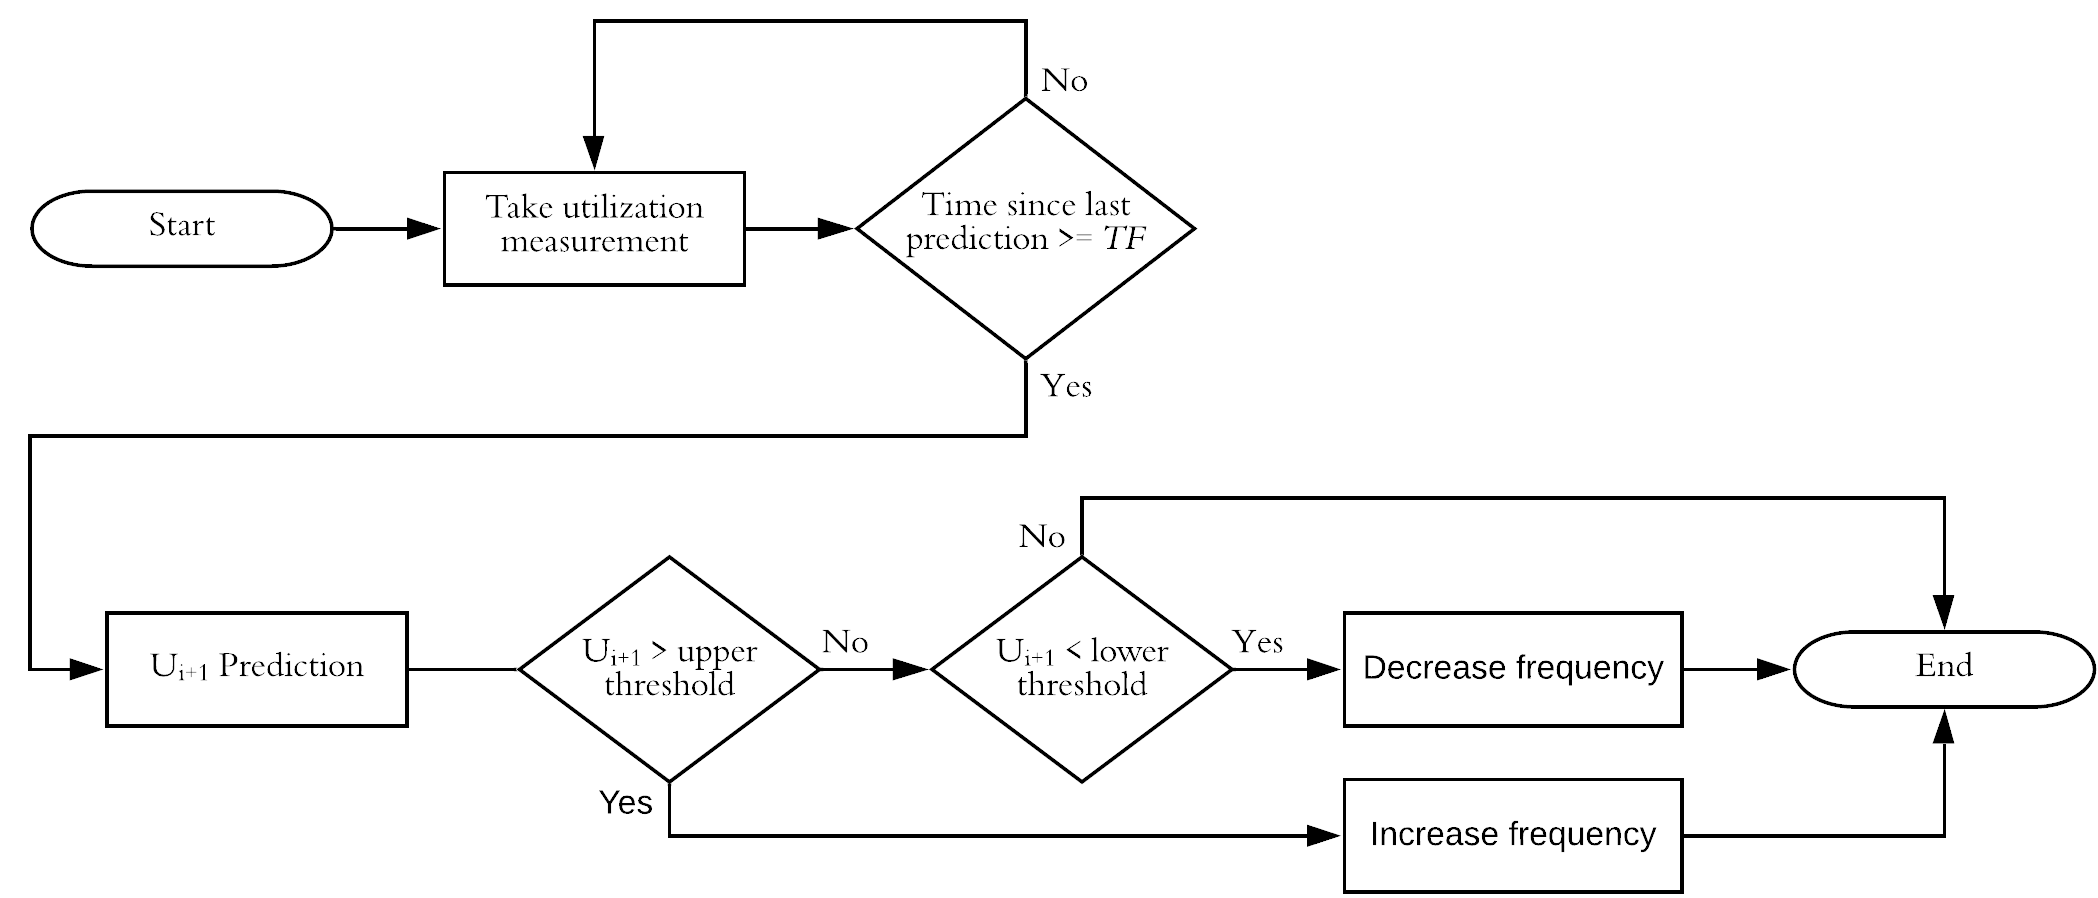
\includegraphics[width=1\textwidth]{Figures/StateArt/DVFSprogram.png}
  \caption[Controller]{DVFS procedure.}
  \label{fig:DVFSprocedure}
\end{figure}

\subsubsection{Task-based}

Task-based DVFS algorithms analyze the source code and the task profiling results (performance counters values) to determine the optimal frequency/voltage. This type of algorithm is composed of an intra-task and an inter-task analysis \cite{noauthor_time_nodate}. The intra-task part decomposes the execution of the task or a process into the on-chip computation and off-chip access latencies. Based on the results,  the optimal GPU core and memory frequency are determined accordingly to the ratio between the two types of execution. Inter-task mechanisms utilize the intra-task results, assigning a signature to each type of task/process. By analyzing, in run-time, the performance counters, and using a lookup table that stores the signatures, the optimal frequency/voltage is set for the sequence of tasks being executed.

In general, the challenges of creating a better GPU DVFS relates to three factors. The GPU power management is very limited, the lack of accurate quantitative GPU DVFS performance and power estimation tools, and the fact that the GPU architecture design is still evolving rapidly, which makes the strategies applied to one architecture design have different outcomes on the next iteration of it \cite{mei_survey_2016}. The observed results show that strategies like scaling up the processor frequency, race-to-idle  \cite{hoffmann_racing_2013} or "racing" \cite{kim_racing_2015}, when a task is launched in the pursuit of finishing it as fast as possible and return to an idle state, prof to increase the energy efficiency of CPUs, however, that assumption not always results in the same outcome for GPUs \cite{kim_racing_2015}. 

\subsubsection{AMD DVFS Mechanism Example}

The control mechanism of the GPU DVFS used nowadays by both AMD and NVIDIA, schematized on figure \ref{fig:DVFSmechanism}, is primarily an interval based one. The most recent AMD GPU DVFS mechanism is called Adaptive Frequency and Voltage Scaling (AVFS) \cite{amd_polaris_nodate}. AFVS takes into account the voltage levels across the different parts of the GPU, the die temperature, the frequency and, the total power consumption. The objective of the controller is to maintain the total power consumption within the required power and temperature envelope, this is, for a given power target, when launching a new task, the GPU tries to achieve the highest possible frequency (highest performance level). For that, it adjusts the voltage level to the one required to correct functioning. With the use of the highest performance level, power and temperature increases, when one of these parameters achieves the limit, the GPU decreases to a lower performance level to maintain itself within the power and temperature target. 

\begin{figure}[!htb]
  \centering
  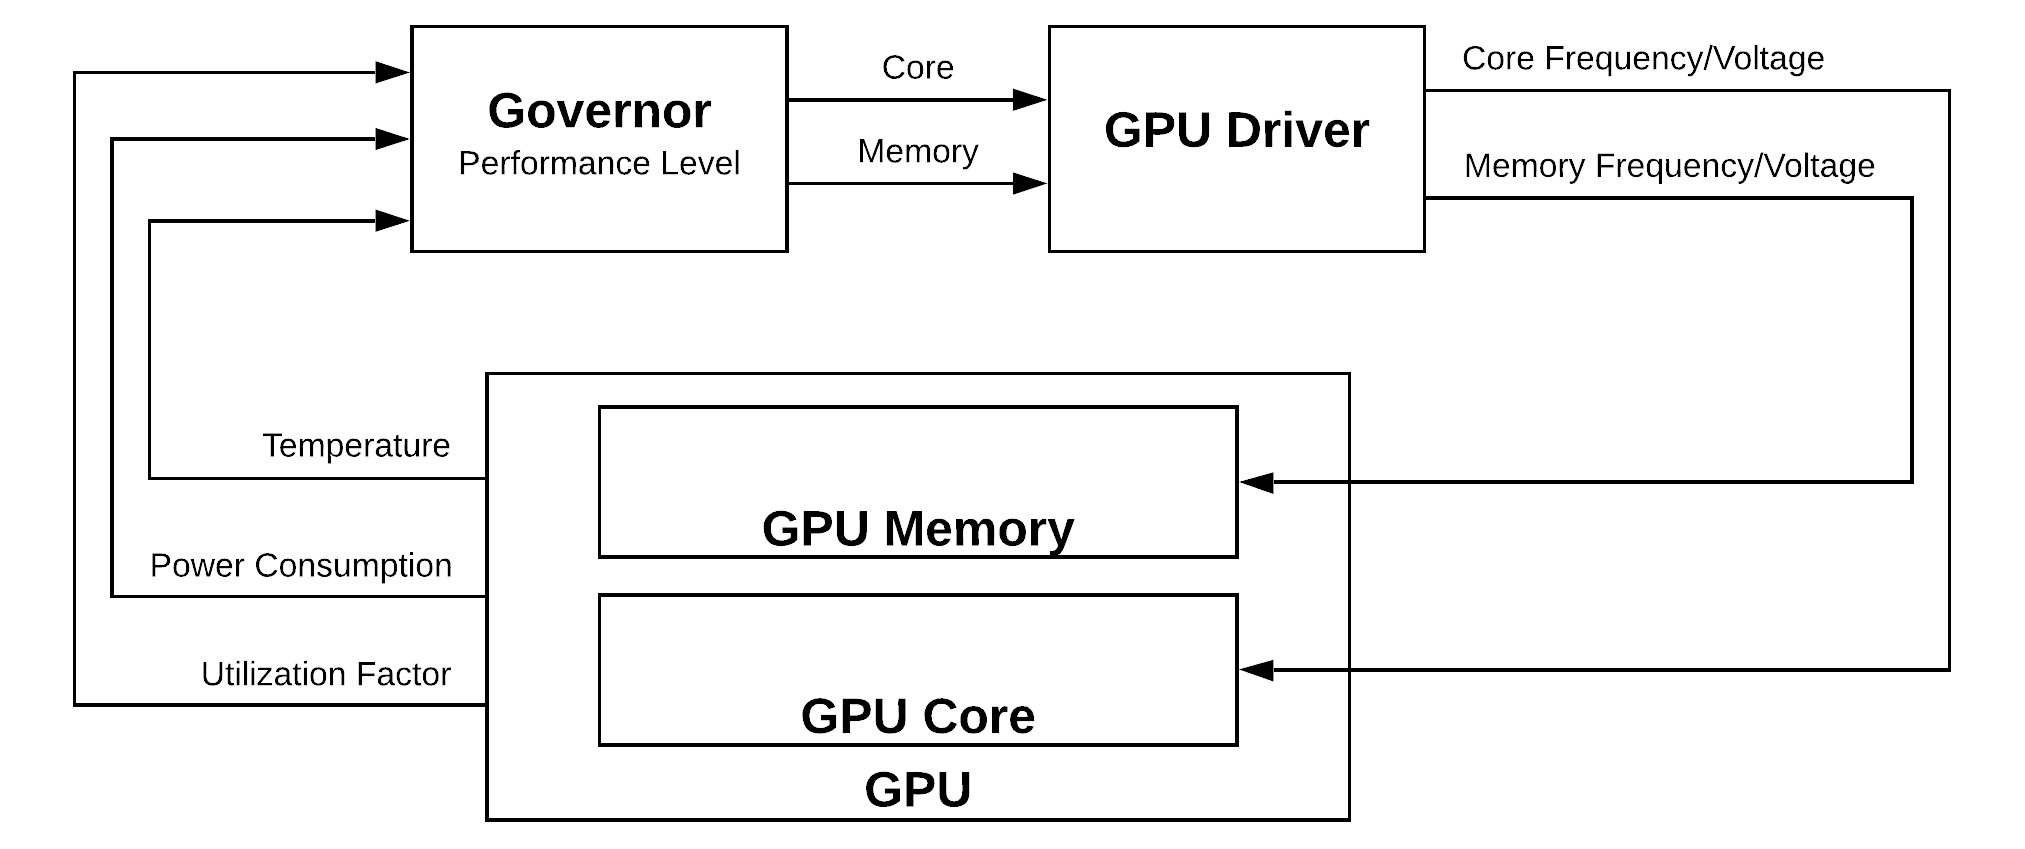
\includegraphics[width=0.8\textwidth]{Figures/StateArt/DVFS.png}
  \caption[Controller]{DVFS control mechanism.}
  \label{fig:DVFSmechanism}
\end{figure}

The major drawback of the current implementation of GPU DVFS is not taking into account the type of task that the GPU is solving. The dominant control mechanism still considers the GPU as a block box and controls its DVFS settings, only looking to outside parameters. Even though the black box approach is enabling significant improvements in current hardware, it lacks the optimization of the frequency/voltage to the type of workload. For instance, a given application can be compute-bound or memory-bound, depending on if the time that it takes to performed is limited by the processor performance or the memory bandwidth and latency. This binary classification of applications also depends on the frequency of the core and memory. The same application can be compute-bounded at a low core frequency, but be memory-bounded at an higher core frequency \cite{guerreiro_dvfs-aware_2019} (the bottleneck switches from the processing elements to the memory). In the case of compute-bounded application, the limitation can be imposed by different components of the processor architecture, depending on the type of data (integer or floats) and the intended precision (size of the operands). If one compares the computation with the same type of operands but with different precision, for instance, 16 vs. 32 bits, even though the GPU is using the same arithmetic unit, the critical path for 32 bits operands is of increased length. That is, the maximum delay between the input and output for operations increases with the precision of the operands. Though, since the same clock frequency is used in both cases, the voltage level needs to be set at a level that ensures that the transistors flip at fast enough rate for the case with the highest precision. Considering that the manufacturers do not tune their devices to the minimum voltage level, to accommodate for manufacturing imprecisions and to leave a safe guardband, the operating voltage of the circuits can be significantly reduced, leading to significant power savings. 

Overall, the minimum operating voltage of each performance level is set at a level high enough, that ensures the correct functioning of the GPU, independently of the computations being performed. Nevertheless, it is possible to better fine-tune the voltage and frequency if the type of task being executed is known.

\subsection{GPU DVFS Characterization and Effects}

Being the GPU such a widely used computation platform, in order to improve their performance and energy efficiency, it is of significant matter the characterization and analysis of the DVFS effects, mainly on understanding the impact of the different parameters on different workloads scenarios. 

A complete GPU DVFS characterization is explored in the literature using two methodologies. The first is experimental studies, where researchers use real GPUs to perform voltage and frequency scaling. Due to past dominance of NVIDIA over AMD \cite{noauthor_jon_nodate} \cite{mujtaba_amd_2019} and the fact that this manufacturer only offers limited support for independent voltage scaling tools, the majority of the work act solely on frequency scaling. The second approach uses simulators, like GPGPU-Sim \cite{noauthor_gpgpu-sim/gpgpu-sim_distribution_2019} and GPUWattch \cite{noauthor_gpu_nodate} \cite{leng_gpuwattch:_2013},  to simulate various scaling approaches like GPU core number scaling and per-core DVFS \cite{mei_survey_2016}. The benefit of using simulators over real hardware comes on the increased flexibility allowed by the previous, enabling the experimentation of scenarios not supported by the frequency/voltage scaling tools provided by the manufacturers. In both methodologies, the studies act on the impact on performance, energy consumption and overall energy efficiency.

\subsubsection{Experimental}

Jiao \textit{et al.} \cite{jiao_power_2010} scaled the GPU core and memory frequency of an NVIDIA Tesla GTX 280 using three types of workload. First, a compute-bounded dense matrix multiplication application, second, a memory bounded application that performs dense matrix transpose and third, a mixed workload, Fast Fourier Transform (FFT) computation. The experimental study showed that for the same core-memory frequency settings, the three applications showed different performance and energy efficiency curves. While a computed bounded application showed to be insensitive to memory scaling, the mixed workload FFT takes advantage of high memory frequency and low core frequency. At last, the memory bounded application profits from both high core and memory frequency. In general, it was shown that energy efficiency could be determined by the instructions per cycle (IPC) and by the global ratio of memory transactions by computation transactions.

Ge \textit{et al.} \cite{ge_effects_2013} explored dense matrix multiplication kernel execution in more detail using an NVIDIA Kepler K20c GPU.  The work revealed that for this type of kernel (compute-bounded), the power used by the GPU and the achievable performance is linear to the GPU core frequency and that the total energy consumption had no relation to frequency scaling. In all the application tests used, the energy efficiency has a linear relation with the GPU frequency, with the highest energy efficiency achieved when the highest clock frequency was employed.

Abe \textit{et al.} \cite{abe_power_2012} introduced a global scaling procedure that combines the GPU core and memory frequency with the CPU frequency in order to minimize energy consumption. In the first experimentation, it was tried to optimize the computation of dense matrix multiplication with differing matrix sizes. Using this global scheme on a small matrix leads to a 28\% energy saving while using low GPU memory frequency and high GPU core frequency. The same procedure was then enlarged to a more diverse set of 33 benchmarks where all the possible combinations of a low, medium, and high GPU core and memory frequency were tested to find the optimal working settings. It was found that energy consumption can be reduced as much as 75\% within a performance loss of 30\% when the best settings were used. 

Mei \textit{et al.} \cite{mei_measurement_2013} conducted a more general experimentation using 37 GPU benchmarks. In this work, it was possible to observe that the effect of GPU DVFS depends on application characteristics. In all situations, the fine-tuning of DVFS per application (finding the lowest voltage level for the desired running frequency) conveyed an energy-saving of 20\%, on average, with only a 4\% performance loss. More recently, Mei  \textit{et al.}, expanded the previous work to analyze the relation between energy consumption and dynamic frequency scaling settings \cite{mei_survey_2016}. For the  Rodinia benchmark \cite{che_rodinia:_2009} it was found that some benchmarks increase the energy consumption linearly with frequency scaling while others are insensitive to the change of this parameter. In the particular case of GPU memory frequency scaling, the work revealed that underclocking this component can result in a 30\% energy decrease if the running application is not memory bounded. For the case of applications that the performance depends on the memory, decreasing the frequency, can lead up to 54\% energy increased due to the increased execution time. In this set of applications, overclocking the memory results in diminishing execution time with reduced overall energy consumption (the small reduction on computation time is overshadowed by the memory energy consumption increase). Overall the relation between the DVFS settings and the energy consumption depends heavily on the application type, and a simple linear model (normally used by the GPU manufacturers) for DVFS settings is inadequate to achieve the best performance or energy consumption/efficiency.


%%%%%%%% EXPERIMENTAL

%ASurveyandMeasurementStudyofGPUDVFSonEnergyConservation
%Jiao et al. scaled the core frequency and the memory frequency of a NVIDIA Tesla GTX280 GPU with three typical applications: the compute-intensive dense matrix multiply, the memory - intensive dense matrix transpose, and the hybrid fast Fourier transform (FFT) [31]. The three applications showed different performance and energy efficiency curves with the same core-memory frequency settings: the dense matrix multiply was insensitive to memory frequency scaling, FFT benefited from low core frequency and high memory frequency, while dense matrix transpose needed both high core and memory frequency. They also found that the energy efficiency was largely determined by the instructions per cycle (IPC) and the ratio of the amount of global memory transactions over the amount of computation transactions. 
%Ge et al. applied fine-grained GPU core frequency and coarse-grained GPU memory frequency on a Kepler K20c GPU, and compared its effect to the CPU frequency scaling [19]. They found that for dense matrix multiply, both the GPU power and the GPU performance were linear to the GPU core frequency, and the GPU energy consumption was insensitive to frequency scaling. For their three tested applications, the highest GPU frequency always resulted in best energy efficiency, differing from the CPU DVFS. 
%In our previous work, we scaled the core voltage, the core frequency and the memory frequency of the Fermi GTX560Ti GPU, with a set of 37 GPU applications [47]. We found that the effect of GPU DVFS depends on the application characteristics. The optimal setting to consume the least energy was a combination of appropriate GPU memory frequency and core voltage/frequency. We observed an average of 20% reduction of energy consumption with only 4% of performance loss. 
%Abe et al. combined the GPU core frequency, the GPU memory frequency and the CPU core frequency scaling together, on the NVIDIA Fermi GTX480 GPU [3]. They performed the frequency scaling with dense matrix multiply of various matrix sizes. They could save as much as 28% of the system energy with a small matrix size, low GPU memory frequency and high GPU core frequency. They then extensively scaled the GPU core and memory frequency of 4 GPU products, including the Tesla GTX285, Fermi GTX460/GTX480, and Kepler GTX680, with 33 popular applications [2]. They set both of the core and memory frequency to low, medium and high values, and searched for theoptimalcore-memoryfrequencycombinationthatoffered the best power efficiency. Surprisingly, they found that, for the Kepler GTX680, the default frequency configuration was never optimal, while the opposite for the Tesla GTX285. They could reduce as much as 75% of system energy within 30% of performance loss, for a compute-intensive workload on the Kepler GPU. Their results suggested that DVFS was even more appealing for recent GPUs.
%YouandChungdesignedaperformance-guaranteedDVFS algorithm for the Mali-400MP GPU on a SoC platform [75]. They found that the GPU utilization ratio was not tightly correlated to the GPU performance, and the ondemand DVFS provided by the SoC system was inadequate by wasting a certain amount of power. 
%Jiao et al. studied the GPU core and memory frequency scaling for two concurrent kernels on the Kepler GT640 GPU [30]. They took a set of kernels from the CUDA SDK andRodiniabenchmarkandmeasuredtheirenergyefficiency (GFlops/Watt) with different core-memory frequency settings. They demonstrated that the concurrent kernel execution in combination with GPU DVFS can improve energyefficiency by up to 34.5%. 

%MAXWELL: The authors of the paper scale the frequency and gather the energy consumption of a set of Rodnia benchmars. They show that some benchs benefict (energy efficiency) from underclocking and others from overclocking. Some apps increase the energy consumption linearly, others are insensitive to frequency, others present an optimal setting. The authors show that underclocking the memory results in great energy consumption increase (due to longer execution time). They conclude that the default setting is the best one. For the few kernels that reduce energy consumption with memory overclock is due to the reduce execution time outshadows the energy increase on the memory
%FERMI: Authors scale down both core clock and voltage, achieve great energy reduction. Best energy at lowest voltage/frequency. Dont find a relation between memory DVFS and energy/performance.
% Appropriate core frequency setting is effective for energy saving. Both platforms expose the “pacing [34]” feature. The relationship between the performance and the GPU core frequency is very complex and a simple linear model is inadequate; 2) In terms of memory frequency scaling, the early platform exposes the “pacing” feature, while the modern platform exposes the “racing [34]” feature. The performance is highly linear to the GPU memory frequency on our Maxwell platform.
%Highly platform /architecture dependent


% A Survey of Methods For Analyzing and Improving GPU Energy Efficiency
%Jiao et al. [2010] study the the performance and power consumption of GPU for three computationally diverse applications for varying processor and memory frequencies. Specifically, they study dense matrix multiplication (compute-intensive), dense matrix transpose (memory-intensive), and fast Fourier transform (hybrid). They have observed that the power consumption of GPUs is primarily dependent on the ratio of global memory transactions to computation instructions and the rate of issuing instructions. These two metrics decide whether an application is memory-intensive or computation-intensive, respectively. Based on these characteristics, the frequency of GPU cores and memory is adjusted to save energy


\subsubsection{Simulation}

As early referred, the characterization of GPU DVFS with simulation is done by using software like GPGPU-Sim \cite{noauthor_gpgpu-sim/gpgpu-sim_distribution_2019} and GPUWattch \cite{noauthor_gpu_nodate} \cite{leng_gpuwattch:_2013}. GPGPU-Sim is an architecture simulator of GPU architecture running CUDA and OpenCL workloads. GPUWattch is an energy model that can predict the energy consumption based on the number of computations and memory access that GPGPU-Sim simulates. Together, both programs can be used to accurately model current and novel GPU architectures and DVFS controllers.

Leng \textit{et al.} \cite{leng_gpuwattch:_2013}, the developers of GPUWattch, simulated the execution of compute and memory-bounded kernels in three scenarios: no DVFS and using a custom off-chip and on-chip DVFS. The custom DVFS algorithm monitors the average number of stall cycles caused by memory operations, when the number increases, the controller switches to a slower performance sate, when the number of stall cycles reduces, the controller places the GPU in a higher performance level. The difference between the on-chip and off-chip DVFS is on time it takes to respond to the number of stall cycles. While the on-chip can switch the performance level in 500 cycles, the off-chip takes 10000 cycles. The results show that using the off-chip DVFS versus no DVFS, results in 13.2\% of energy savings, on average, and using the on-chip DVFS yield a 14.4\% energy saving.

Cha \textit{et al.} \cite{cha_core-level_2018} use GPGPU-Sim to create a GPU core space-multitasking simulator, where per-kernel dynamic frequency scaling (acting on the computing unit level) settings can be applied in concurrent kernel execution. They used Rodinia suite \cite{che_rodinia:_2009}, Parboil suite \cite{stratton_parboil:_nodate}, and Polybench suite \cite{noauthor_polybench/c_nodate} of benchmarks and combine the execution of different kernels, creating pairs of two compute-bounded (Com + Com) kernels, one compute-bounded plus one memory-bounded kernel (Com + Mem) and two memory-bounded kernels (Mem + Mem). The work evaluated the performance of the GPU by measuring the number of executed instructions per second. It was shown that for Com + Com concurrent kernel execution, the performance is linear to the per-kernel DVFS setting. An increase of 20\% on the DVFS of both kernels, results in a 20.4\% performance increase, while a 20\% decrease, results in a 19.3\% decrease in performance. For Mem + Mem concurrent kernel execution, the performance did not change significantly with the changes on the DVFS. The more interesting case is where mixed (Com + Mem) type kernels are concurrently executing. In this case, the per-kernels DVFS can overclock the CU of the Com kernel while underclocking the ones running the Mem kernel, in this setup, the highest performance is achieved for the Com kernel, and the energy (even though was not the objective of the work) is minimized.

%%%%%%% SIMULATION

%ASurveyandMeasurementStudyofGPUDVFSonEnergyConservation
%In [37], Lee et al. simulated the GPU DVFS as well as the core number scaling in GPGPUSim, based on the 32nm prediction technology model [78], with the objective to improve the throughput. Their scaling scheme can provide an average of 20% higher throughput than the baseline GPU. 

%Leng et al. developed GPUWattch, which could simulate the cycle-level GPU core voltage/frequency scaling, based on the Fermi GTX480 GPU [38]. They configured the various GPU voltage/frequency settings according to the 45nm prediction technology model [78], [10], and simulated both slow off-chip and prompt on-chip DVFS. They gained an average of 13.2% energy saving with off-chip DVFS and 14.4% energy saving with on-chip DVFS, both within 3% performance loss. For either scaling scheme, they found that the memory-bounded kernels benefited a lot but the purely compute-bounded kernels did not take much advantage of the DVFS. 




%Core-level DVFS for Spatial Multitasking GPUs 
%It is difficult to analyse DVFS when in spatial multitasking, and determine the optimal DVFS. Created GPU simulatoor, operates DVFS at the SM level
% They used Rodinia suite[6], Parboil suite[5] and Polybench suite [7]. benchs and combine (Com + Com), (Mem + Mem), and (Mem + Com)  apps , measure IPC for perforamce metric becasuse the clock period of one cycle varies when the frequency changes. 
%Com+ COM - Executing two computeintensive kernels with a 20 % increase in the SM frequency (in the case of H+H) resulted in a 20.4% increase in the performance compared with the baseline (N+N). Conversely, when the SM frequency was reduced by 20% (L + L), the performance was reduced by 19.3% compared with the baseline. performance has been changed linearly by the frequency of the SM where the kernel is running
%2) Mem+Mem Cases -  the performance did not change significantly depending on the SM frequency
%3) Mem+Com Cases : By increasing the frequency of all SMs by 20% (H + H), the performance of the memory-intensive kernels increased only by 3.7% compared with the baseline but the performance of the computeintensive kernel increased by 11.5%. For the (L + L) case, the performance of the memory-intensive kernel and the computeintensive kernel decreased by 5.8% and 17.3%, respectively. The performance of the (H + N) case was similar to the baseline. The performance of the (H + L) case was similar to that of the (N + L) case. In the (Mem + Com) configuration, the performance of compute-intensive kernel in the (N + H) case was the best, which improved the performance by 17.4% compared with the baseline. This performance gain is higher than that of the (H + H) case and power consumption is also expected to be less.  
 %Over and underclock of 1/4 - draw back is the added hardware




\subsection{DVFS Optimization}

As induced by the works presented in the previous section, by correlating the DVFS parameters with the application characteristics, it is possible to improve the performance and reduce the energy consumption of GPU accelerated programs.  The investigation on new DVFS mechanisms acts on two fronts: enabling finer-grained DVFS control, with the creation of more clock/voltage domains within each GPU component, and on the creation of novel DVFS control mechanisms, searching how can more sophisticated and aware DVFS systems,  better control the voltage and frequency depending on the workload type.

Sethia \textit{et al.} \cite{sethia_equalizer:_2014} designed \textit{Equalizer}, a low overhead hardware runtime system, able to dynamically perform the monitorization and management of GPU resources and kernel requirements. This mechanism is placed in the instruction decoder pipeline attached to the kernel scheduler (scoreboard control mechanism that indicates which kernel should be run and where). By controlling the on-chip concurrency and core and memory frequency, they are able to create two running modes based on four counter utilization values (number of active and waiting threads, and number of ALU and memory instructions). In energy mode, it achieves 15\% savings in energy, while in performance mode, it is able to increase the performance by 22\%.

Thomas \textit{et al.} \cite{thomas_application_2018} proposed Application aware Scalable Architecture (ApSA) for GPGPU applications. ApSA is a three-stage runtime hardware profiling and scheduler mechanism able to adjust the working of the GPUs core depending on the category of the application. On the first and second stage, profiling and decision-making, ApSA classify applications as of type-I or type-II. An application is classified as type-I if it requires more processing cores to increase the performance and of type-II, if it needs more performance of the memory system to run faster. Accordingly to the classification, on stage three, action, the ApSA mechanism will make the application run on all available CU if it is of type-I. If it is of type-II, the proposed mechanism only indicates that half of the available threads should run the application. At the same time, the frequency controller scales down the core and scales up the memory frequency, increasing the energy efficiency of the GPU. By running the ApSA mechanism, a profiling overhead of 1.6\% for type-I applications and 1.15\% for type-II is introduced. Nevertheless, a reduction of 20.08\% of power is achieved by using the ApSA mechanism.

Akiki \textit{et al.} \cite{akiki_energy-aware_2018} proposes a run-time gradient descent (GD) optimal frequency search algorithm. This mechanism relies on the target application be run multiple times and in each iteration, an exploration of the frequency is made. By indicating the target metric, such as performance or energy-delay product (EDP), it is possible to validate if the new frequency is better than the earlier one. By running this procedure alongside a set of benchmarks, with EDP selected as the target metric, it was achieved a reduction of 15\% on energy consumption.

Huang \textit{et al.} \cite{huang_gpu_2019} introduced an novel proportional-integral-derivative neural network (PIDNN) frequency controller. This controller uses gradient descent to find the most appropriate frequency to be applied to the GPU core, memory and interconnect network in order to reduce energy consumption. The designed neural network has as input the current frequency of each GPU component and the number of kernels to be dispatched, the interconnect message queue size and the number of caches misses. The hidden layers of the neural network represent proportional-integral-derivative controllers and the output layer corresponds to the new frequency to be set on the core, memory and interconnect. After the model is trained, depending on the GPU model, the novel DVFS controller can reduce energy consumption between 4.39\% and 18.67\% on the tested benchmarks.

In the work of Cha \textit{et al.} \cite{cha_core-level_2018} presented earlier, it is discussed how does the application of DVFS at the CU level improve the performance and the energy consumption of the GPU. Using the GPGPUSim GPU simulator, they created a multiclock generator able to provide a fast, base and slow clock to each of the CU at demand.  By reserving a register on each CU, that the compiler will write to with the information regarding what is the most appropriate clock frequency, each CU will inform the multiclock generator which of the three clocks should be active. By enabling this finer-grain DVFS, it made it possible for the acceleration of computed-bounded kernels while still providing the most energy efficiency frequency to those how are memory-bounded.




%Sethia et al. designed a dynamic runtime GPU core number, core and memory frequency scaling system, to either conserve the energy or improve the performance [64]. They categorized the GPU applications into 3 types: computeintensive, memory-intensive, and cache sensitive, according to GPUWattch characterizations. For each application category and scaling objective, they designed different scaling strategies. Their system reduced 15% energy in the energysaving mode. 
%Sen et al. applied the fine-grained per-core DVFS in GPUWattch, in view of the diverse execution time and workload of different GPU cores [63]. They found the percore DVFS had good potential to save more power than the overall DVFS. 

%Clock splitting technique
%grande margem para fazer tudo, nao optimizado

%Aggressive Voltage and Temperature Control for Power Saving in Mobile Application Processors
%Study the effects of a temperature aware DVFS on mobile devices to relate with the TEMPERATURE INVERSION PHENOMENON 
%We demonstrated that the T-DVS can achieve power saving with aggressive voltage control by capitalizing on the relationship between operating voltage and temperature. We expect the T-DVS to set a milestone in active voltage control for power management in mobile devices. The effectiveness of the T-DVS was achieved solely by using software approaches and employing existing hardware features. 

%Motivated by the fact that scaling down the core voltage was vital to conserve energy, Gopireddy et al. designed a new architecture that enabled a lower operating voltage in the energy-efficiency mode other than the normal voltage in the high-performance mode [23]. Their simulation results showed that the new hardware could reduce as much as 48% of energy consumption, compared to the conventional hardware with normal DVFS. In summary, GPU DVFS is proved to be effective in energy conservation for a variety of applications, but the impact on different applications are very diverse. Researchers need to design specific scaling algorithm based on the application characteristics. 



%GPGPU-Perf: efficient, interval-based DVFS algorithm for mobile GPGPU applications
% GPUs can be used to two types of workloads, graphics and GPGPU. In graphics, there's a objective of 30/60 fps to be met, when over performance is available, we can decrease the F and V. However, in GPGPU, GPU should process them as fast as possible. They create a new GPGPU-Perf algorithm that adjusts the DVFS params (threshold and interval) which results performance over energy increases by 1.44 times with no influences on graphic tasks and any modifications of GPGPU algorithms.
% They expand OpenCL to include a DVFS programming interface. If only a single set of thresholds is available regardless of the presence of graphic or GPGPU tasks, it makes sense thatgraphicapplicationshaveahigherprioritythanGPGPU applicationstodeterminethethresholds, HU and HD,mainly because the number of existing graphic applications in the fieldsismuchhigherthanthatofGPGPUapplications.
% weighted thresholding based on working times, adaptive interval adjustment based on utilization changes and multi-level frequency adjustment based on previous utilization. he performance 2.04 times with energy consumption 1.51 times via intelligent frequency controls.

 



%%%%%%%%%%%%%%%%%%%%%%%%%%%%%%%%%%%%%%%%%%%%%%%%%%%%%%%%%%%%%%%%%%%%%%%%
\section{Models}
\label{section:Models}
%%% ALTERAR A ORDEM DE TOP DOWN e BOTTOM UP para ficar todos pela mesma ordem
To be able to predict, beforehand, the best voltage and frequency for a given workload, a power and performance model has to engineered that reflects the GPU workings. The models can be constructed using either a top-down or a bottom-up approach, depending on if they look into the GPU architecture and the running kernel to modulate, or if they look onto the runtime performance models to acquire knowledge about what the device is computing.

\subsection{Power Modeling}
\label{subsection:powermodels}

Power models try to predict the power and energy consumption of the GPU over the computation of a given application. The power modeling can be done using either empirical or statistical methods. The former relies on the binary code analysis, performing a bottom-up approach where the GPU-microarchitecture needs to be known for the prediction of the power. The later uses perform a power analysis relying upon the performance counters, this top-down approach treats the GPU as a black-box and seeks and establishes relationships between the GPU power and the runtime performance counters \cite{mei_survey_2016}.

\subsubsection{Empirical Methods}
\label{subsubsection:EmpiricalMethods}
The empirical power modeling of processor started with CPU modeling, back on the Pentium 4 era, where Isci and Margaret introduced the first empirical power modeling techniques \cite{isci_runtime_2003}. The proposed method decomposes the processor into separated hardware components, and by estimating the maximum power consumption of each component (based on the architecture and utilization factor), the total power consumption is computed as the sum of all components. Equation \ref{eq:empiracalPower} reflects the mathematical model of the total power consumption of the device as the sum of $P_0$, a constant power factor, plus all its \textit{n} subcomponents power and utilization rates. 

\begin{equation}
\label{eq:empiracalPower}
    P = P_0 + P_1 * r_1 +  P_2 * r_2 + ... + P_n * r_n
\end{equation}

Hong and Kim first applied this modeling method for the GPUs \cite{hong_integrated_2010}. The authors started by creating an examination mechanism that analysis the PTX code (assembly instructions of the NVIDIA GPUs) to estimate, based on the number of instructions and pipeline analysis, the utilization rate of each of the GPU separated units. To find out the \textit{P} values of each of the GPU separated units, a suite of benchmarks was designed to give the minimum error between the computed and measured power. Given all the \textit{P} values to the model of Equation \ref{eq:empiracalPower} and getting the utilization rate from the examination mechanism, they were able to achieve a 2.5\% power prediction error for micro-benchmarks and 9.2\% for integrated GPGPU kernels.

Based on Hong and Kim's work and on the GPGPUSim GPU simulator, Leng \textit{et al.} created the before mentioned GPUWattch simulator \cite{noauthor_gpu_nodate} \cite{leng_gpuwattch:_2013}. This simulator uses empirical methods to estimate the runtime GPU power for different frequency and voltage settings. 

The leading critic of this modeling method is that it is product-specific, with the \textit{P} values and the assembly examination tool not being easily ported from one GPU architecture to others. Other researchers introduced more straightforward empirical modeling techniques based on per-core execution time and the number of instructions per cycle achieved by the architecture that also achieves upwards of 90\% accuracy on predicting the power while being much more easily ported between different GPUs \cite{mei_survey_2016}.

\subsubsection{Statistical Methods}
\label{subsubsection:StatisticalMethods}

Statistical power modeling methods can predict the power consumption of the GPU by analyzing the runtime performance counters of GPU accelerated applications with monitor software. This top-down approach considers the GPU micro-architecture a black box. By training and fitting power model with the runtime power consumption and micro-architecture events, it is possible to characterize the GPU power consumption for different workloads.

The power models are based on mathematical and machine learning models that can be broken in linear and non-linear models. Linear models, more straightforward, and the first being used include support vector regression (SVM), square linear regression, random forest, and generalized additive model.
Given a set of $x_n$ input variables (performance counters, runtime power consumption), the linear trained model predicts the total power consumption by applying Equation \ref{eq:statisticalPower}, where $a_n$ represents the output contribution of each input variable.

\begin{equation}
\label{eq:statisticalPower}
    P = a_0 + a_1 * x_1 + a_2 * x_2 + ... + a_n * x_n
\end{equation}

Non-linear models such as artificial neural networks (ANN) and K-means can coup with more complex relationships and are gaining popularity for the increased accuracy that they provide \cite{mei_survey_2016}. 

Examples of the application of statistical are found throughout the literature. Nagasaka \textit{et al.} \cite{nagasaka_statistical_2010} used square linear regression to predict the power consumption of the Rodinia benchmark suite \cite{che_rodinia:_2009}, the fitted model predicts that the constant part $a_0$ counts for 70\% of the power consumption and that, besides that factor, the instruction count and the global memory accesses contribute the most to the GPU runtime power.  Chen \textit{et al.} \cite{chen_statistical_2011} used a random forest model in combination with the GPGPUSim GPU simulator, which could decode the kernels to separated hardware instructions, to predict the power consumption of Rodinia \cite{che_rodinia:_2009} and Parboil suite \cite{stratton_parboil:_nodate} benchmark suites. The results suggested that the registers, single-precision floating-point, global memory, integer and arithmetic logic instructions were the most influential variables. The most recent works using linear models, like \cite{abe_power_2014} and \cite{ghosh_statistical_2013}, can achieve up to 85\% of accuracy.

The use of non-linear models allows the gathering of non-linear relationships between the input variables and the output and the cross-impact of multiple input parameters. Song \textit{et al.} \cite{song_simplified_2013} trained the GPU runtime power with an ANN of two hidden layers for the same benchmarks as Nagasaka \textit{et al.} \cite{nagasaka_statistical_2010} and Chen \textit{et al.} \cite{chen_statistical_2011}, achieving accuracy above 93.3\% in all benchmarks. More recently, Wu et al. \cite{wu_gpgpu_2015} and Dutta et al. \cite{dutta_gpu_2018} generalized the power prediction models using machine learning to predict the power consumption of the GPU at diverse DVFS settings. Wu et al. focused on kernels, while Dutta et al. can predict at a higher level with complete applications. Both works achieve accuracy above 96.5\% in their power statistical models. These works prove that non-linear models can outperform linear ones and achieve better model predictions.

In general, the use of these types of statistical analysis allows for the understanding of the most critical factors on GPU power consumption.    

\subsection{Performance Modeling}
\label{subsection:performancemodels}

Performance models predict the performance with the operating frequency scaling of the GPU core and memory. Similarly to power models, Subsection \ref{subsection:powermodels}, performance models can use a top-down or a bottom-up approach. Statistical Methods uses a top-down approach, where performance counters are analyzed to found possible bottlenecks and the runtime throughput of the device, on the other side, pipeline analysis, a bottom-up approach, requires the previous knowledge of the GPU execution principals and an analysis of the application to be run, in order to predict the performance metrics \cite{mei_survey_2016}. 

\subsubsection{Pipeline Analysis}
Performance modeling by pipeline analysis is performed by assembling the GPU execution and memory pipeline and analyzing the computation/memory parallelism \cite{mei_survey_2016}. The performance of the GPU can be taken by evaluating different metrics such as MWP, CWP, or LCP. MWP - memory warp parallelism looks into the maximum number of sets of threads (warps) of one CU, that can access the memory concurrently during the \textit{memory waiting period} - time taken by the warp memory request to be launch and returned. CWP - computation warp parallelism examines the number of warps that one CU can execute during the time that the \textit{memory waiting period} takes. LCP - load critical path examines the most extended sequence of dependent memory loads that are possible to overlap with computations from parallel warps. All the presented methods analyze the behavior of the architecture (core + memory) to critical computing situations, allowing for the determination of the maximum available performance.

\subsubsection{Statistical Methods}
The performance modeling using statistical methods is analogous to the power modeling technique where runtime performance counters are used to determine the behavior of the device for different workloads and DVFS scenarios. Both linear and non-linear models are fitted or trained with architecture runtime events of benchmarks that stress the different components of the GPU (core and memory). By breaking down the applications to be analyzed on their fundamental types of computations (extracted by performance counters reports of previous runs), it is possible to predict the achievable performance for different DVFS settings. One of the best examples of performance modeling using this methodology is the work of Wu \textit{et al.} \cite{wu_gpgpu_2015}. In this work, the performance of an AMD GPU is modeled for different core and memory frequencies. The model is based on K-means clustering an ANN, achieving an average error of performance prediction of 15\% across the working frequency range.

The state of the art of modeling techniques for power and performance use similar techniques, however, comparing the prediction accuracy for the two metrics, the power models can achieve more closer to life results than performance models. This can be a challenging factor for the creation of DVFS aware strategies that want to optimize energy efficiency (performance/power) rather than power or performance solely.

\section{Related Work}

The presented state of the art on DVFS exploration, characterization and modeling methodologies explored the benefits of using mainly frequency scaling in order to optimize the performance and reduce the power consumption on GPUs. However, the significant frequency and voltage guardbands used by manufacturers, to ensure the correct functioning of the devices across all possible working conditions, appear to be an extra beneficial space that is waiting to be explored.  In that regard, more recent studies have been playing not only with frequency, but also with voltage scaling beyond the conventional DVFS limits. The studies presented in the section show that working in this unexplored space can be profitable when certain conditions are present.

To beneficially use voltage scaling outside conventional DVFS limits, it is necessary to understand how does the size of the voltage guards and the minimum operating voltage - $V_{min}$, relate to the different types of applications. The work of Leng \textit{et al.} \cite{leng_safe_2015} contributes by analyzing the voltage guardband of different applications and by creating a statistical analysis procedure to predict the $V_{min}$ depending on collected performance counters. For the voltage guardband analysis, Leng \textit{et al.} used 57 representative programs which are run on four different GPUs of two different architectures. The testing procedure consists of running each program 1000 times, after which a $12mV$ undervoltage is performed on the GPU core if every run is successful, repeating the procedure until a fault occurs. The faults can be of two types: runtime error, such as segmentation fault, silent data corruption or OS crash, and incorrect output (the results of the undervolt run being different from the run with default voltage).  The most significant finding is that across the suite of tested programs, the $V_{min}$ level is at a relatively large (0.1V - 9.2\% to 0.2V - 18.3\%) percent of the conventional minimum operating voltage level (nominal voltage - 1.09V for the tested cards), allowing for a reduction on energy consumption of up to 25\%. However, in order to successfully use the GPU in an undervoltage scenario, it is necessary to understand what, in the architecture and on the application, determines the size of the voltage margin and the $V_{min}$ 

The voltage margin's primary purpose is to guarantee the correct functioning of the GPU against the process, voltage (noise) and temperature (PVT) variation and device aging.
The process variation results from imperfections on the lithography and dopants diffusion. This phenomenon can occur intra-die when devices from the same die present different features depending on its locations, and inter-die, meaning that devices from one die can present different features from devices from another batch of dies. The process variation affects the speed of transistors and overall circuit characteristics by varying the device threshold and speed. In order to guarantee the correct execution of the device at the intended frequency, is necessary to boost the voltage applied to all transistors \cite{thomas_core_2016}.
Leng tested the influence of process variation by running the set of benchmarks on multiple GPUs of the same model, achieving a maximum variability of 0.07V for the same benchmarks. To test the effect of temperature, all the benchmarks were run at 40ºC and 70ºC core temperature. Measuring the $V_{min}$ in both conditions led to 0.02V variation between the runs. The  $V_{min}$ variation for process and temperature has a relatively uniform impact across all programs and it is not sufficiently large to be leading root determining the guardband size. The variability of aging was not possible to measure directly; however, it is plausible to assume that this effect should produce a similar contribution to process and temperature variation \cite{leng_safe_2015}.

Since the process and temperature variation and device aging, seem not to have sufficient impact, by themselves, to explain the variability of $V_{min}$, voltage noise appears to be the leading cause of this variation. Voltage noise is mainly induced by $di/dt$ droop. This phenomenon makes the actual measured voltage applied to the GPU components, Equation \ref{eq:Vactual}, depend on the rate of change of the current being drawn. 

\begin{equation}
    \label{eq:Vactual}
    V_{actual} = V_{DD}-L*\frac{di}{dt}
\end{equation}

The workload intensity variation in runtime induces the $di/dt$ droop due to the rapid and significant change in current demand from the various functional blocks \cite{thomas_core_2016}. A program that induces a bigger $di/dt$ droop will have a smaller voltage margin (superior $V_{min}$). With so, from an analysis of the running application and the type and rate of change of the workloads, it is possible to predict if an application will have a bigger or smaller voltage margin (the difference between GPU nominal voltage and the actual application $V_{min}$).

Works, such as of Leng \textit{et al.} \cite{leng_safe_2015} and Nakhaeea  \textit{et al.} \cite{nakhaee_lifetime_2018} propose methods to determine the $V_{min}$ with different objectives. While Leng aspires to reduce energy consumption, Nakhaeea expects to improve the lifetime of processors. These two examples are only a few of the possible benefits that the exploration of the voltage scaling brings. To model $V_{min}$, Leng used performance counters measurements to train an ANN that predicts the amount of possible undervolt. The root mean square error (RMSE) between the model prediction and the measured result is 0.5\%, with the maximum over and underprediction error of 3\% and 2\%, respectively. The trained ANN is able to correctly model the variation of $V_{min}$ with the type of workload.

In general, a good model of the minimum operating voltage should be able to not only correctly predict  $V_{min}$ across a significant large set of applications, but also minimize the under and overprediction of this value. Overpredicting $V_{min}$ will most likely lead to the occurrence of program faults, and underpredicting the voltage is not using the benefit of this finding at their most.

The study of Tan \textit{et al.} \cite{tan_combating_2016} explored the effects of using low supply voltage on the GPU register file. Demonstrating that this component is one of the most affected and one of the first provoking program faults when not enough voltage is provided. Tan modeled how different voltage levels are impacted by the process variation of the register file, and presented an architectural solution that by taking advantage of register dead time for reliable operations from unreliable register files at low voltage. 

To take advantage of non-conventional voltage scaling, the problem needs to be tackled on the two presented forms. By both analyzing the minimum required voltage and the size of the guardband, and by studying architecture improvements that can improve the reliability of GPU components at low supply voltage. However, if one uses imprecision tolerant applications, it becomes possible to run GPUs at $V_{min}$ with extra confidence that errors induced by low supply voltage will not cause errors on the application's output. This type of application allows the use of techniques such as timing error propagation (TEP) \cite{nakhaee_lifetime_2018}, where computation errors can be propagated to subsequent logic stages with the expectation that the algorithm itself is able to recover from it.

A common application that is taking, nowadays, great advantages of GPU acceleration is Deep Learning (DL). One of the most important characteristics of this type of algorithms is their imprecision tolerance. The computation of a DL application is an iterative and convergence process, and by the natural adaption of the neural networks learning parameters in runtime, the occurrence of small computation errors do not affect the end prediction of the algorithm \cite{jiao_assessment_2017}.

Tang \textit{et al.} \cite{tang_impact_2019} studied the impact of DVFS parameters on the energy and performance of DL applications. Even though the DVFS exploration only used the default range of frequency and voltage scaling, by tunning the parameters, it was possible to either improve the performance by up to 33\% or reduce the energy consumption by 23.1\%. The work applied the same pair of frequency and voltage throw out the complete training or inference session, however, the authors point out that the different layers that compose a neural network can have different voltage and frequency optimizations points. Moreover, by using the inherent resilience of neural networks, it could be possible to find even better working parameters outside of the conventional DVFS range. To summarize, the creation of a DVFS Deep Learning Aware controller, able to adapt the DVFS parameters to the need of each neural network layer, can achieve even further performance and energy efficiency improvements, being exactly this point, the main objective of this thesis.